\documentclass[11pt,a4paper,titlepage]{article}
\usepackage[a4paper, margin=1.25in]{geometry}
\usepackage[utf8]{inputenc}
\usepackage{amsmath}
\usepackage{amsfonts}
\usepackage{amssymb}
\usepackage{graphicx}
\usepackage{float}
\setlength\parindent{0pt}
\usepackage{hyperref}
\hypersetup{
	colorlinks=true,
	linkcolor=blue,
	filecolor=blue,
	urlcolor=blue,
}

\begin{document}
	\title{AMB Design Spreadsheet Equations}
	\author{Ari Meles-Braverman}
	\date{Version 1.1}
	\maketitle
	
	\section{General Motor Equations}
	\subsection{Motor System Equations}
	$\tilde{x}$ denotes the property of a system of equivalent motors connected 1:1 in a gearbox
	\begin{equation}
		\tilde{\omega_f} = \omega_f \cdot \left( \frac{V}{V_{spec}} \right)
	\end{equation}
	\begin{equation}
		\tilde{\tau_s} = \tau_s \cdot \eta n \left( \frac{V}{V_{spec}} \right)
	\end{equation}
	\begin{equation}
		\tilde{i_f} = i_f \cdot n \left( \frac{V}{V_{spec}} \right)
	\end{equation}
	\begin{equation}
		\tilde{i_s} = i_s \cdot n \left( \frac{V}{V_{spec}} \right)
	\end{equation}
	\begin{equation}
		P = \frac{2\pi \omega_f \cdot \tau_s}{4}
	\end{equation}
	\begin{equation}
		\tilde{P} = \frac{2\pi \tilde{\omega_f} \cdot \tilde{\tau_s}}{4} = P \cdot \eta n \left( \frac{V}{V_{spec}} \right) ^2
	\end{equation}
	\begin{equation}
		K_T = \frac{\tilde{\tau_s}}{\tilde{i_s} - \tilde{i_f}}
	\end{equation}
	
	$\omega_f$ = Motor Free Speed \\
	$\tilde{\omega_f}$ = Adjusted Free Speed \\
	$\tau_s$ = Motor Stall Torque \\
	$\tilde{\tau_s}$ = Adjusted Stall Torque \\
	$i_f$ = Motor Free Current \\
	$\tilde{i_f}$ = Adjusted Free Current \\
	$i_s$ = Motor Stall Current \\
	$\tilde{i_s}$ = Adjusted Stall Current \\
	$P$ = Motor Power \\
	$\tilde{P}$ = Adjusted Motor Power \\
	$n$ = \# of Motors \\
	$\eta$ = Gearbox Efficiency \\
	$V$ = Applied Voltage \\
	$V_{spec}$ = Specification Voltage (Almost Always 12) \\
	$K_T$ = Motor Torque Constant
	
	\subsection{Instantaneous Motor Equations}
	\begin{equation} \label{motor_instant_speed}
	\omega = \tilde{\omega_f} \cdot (1 - \frac{\tau}{\tilde{\tau_s}})
	\end{equation}
	\begin{equation} \label{motor_instant_current}
	i = (\tilde{i_s} - \tilde{i_f}) \frac{\tau}{\tilde{\tau_s}} + \tilde{i_f}
	\end{equation}
	\begin{equation} \label{motor_instant_eff}
	\eta_{motor} = \frac{W_{out}}{W_{in}} = \frac{\tau \cdot \omega (\tau)}{V \cdot i (\tau)} = \frac{\tau (\tilde{\tau_s} - \tau) \tilde{\omega_f}}{V (\tilde{i_s} \tau + \tilde{i_f} (\tilde{\tau_s} - \tau))}
	\end{equation}
	
	$\omega$ = Instantaneous Motor Speed \\
	$\tau$ = Instantaneous Motor Torque \\
	$i$ = Instantaneous Motor Current \\
	$\eta_{motor}$ = Instantaneous Motor Efficiency
	
	\section{Mechanism Gear Ratio Calculator}
	\subsection{General Equations}
	\begin{equation}
		\omega_{free} = \frac{\tilde{\omega_f}}{G}
	\end{equation}
	\begin{equation} \label{stall_force}
		F_s = \frac{\tilde{\tau_s} G}{r}
	\end{equation}
	\begin{equation}
		\omega_{load} = \omega_{free} \cdot (1-\frac{F}{F_s})
	\end{equation}
	\begin{equation}
		v_{free} = \omega_{free} \cdot 2\pi r
	\end{equation}
	\begin{equation} \label{wheel_lin_rot}
		v_{load} = \omega_{load} \cdot 2\pi r
	\end{equation}
	\begin{equation} \label{current_per_motor}
		i = \frac{r F}{K_T G n} + \frac{\tilde{i_f}}{n}
	\end{equation}
	\begin{equation} \label{stall_volt}
		V_s = V_{spec} \frac{r F}{\tilde{\tau_s} \eta n G}
	\end{equation}
	
	$G$ = Gear Ratio \\
	$\eta$ = Gearbox Efficiency \\
	$n$ = \# of Motors \\
	$F$ = Load Applied \\
	$r$ = Load Radius \\
	$\omega_{free}$ = Output Rotational Free Speed \\
	$\omega_{load}$ = Output Rotational Loaded Speed \\
	$v_{free}$ = Output Linear Free Speed \\
	$v_{load}$ = Output Linear Loaded Speed \\
	$i$ = Current Per Motor \\
	$F_s$ = Stall Load \\
	$V_s$ = Stall Voltage
	
	\subsection{Gear Ratio Calculations}
	\subsubsection{Maximum Power}
	\begin{equation}
		F_s = 2 F
	\end{equation}
	
	Substituting into (\ref{stall_force}) and solving for $G$ gives:
	\begin{equation}
		G = \frac{2 r F}{\tilde{\tau_s}}
	\end{equation}
	
	\subsubsection{Maximum Efficiency}
	\begin{equation} \label{max_eff}
		G = \frac{r F}{\tilde{\tau_s}} \left( 1 + \sqrt{\frac{\tilde{i_s}}{\tilde{i_f}}} \right)
	\end{equation}
	For derivation, see Appendix \ref{appendixA}
	
	\newpage
	\subsubsection{At Stall}
	\begin{equation}
		F_s = F
	\end{equation}
	
	Substituting into (\ref{stall_force}) and solving for $G$ gives:
	\begin{equation}
	G = \frac{r F}{\tilde{\tau_s}}
	\end{equation}
	
	
	\subsubsection{By Rotational Speed ($\omega_{load}$)}
	We can substitute (\ref{motor_instant_speed}) and (\ref{motor_instant_current}) into (\ref{motor_instant_eff}):
	\begin{equation}
	\omega_{load} = \frac{\tilde{\omega_f}}{G} \cdot (1 - \frac{F}{\frac{\tilde{\tau_s} G}{r}})
	\end{equation}
	
	Solving for G, we get:
	\begin{equation} \label{by_rot_speed}
		G = \frac{\tilde{\omega_f}}{2 \omega_{load}} \left( 1 + \sqrt{1 - 4 r F \frac{\omega_{load}}{\tilde{\tau_s} \tilde{\omega_f}}} \right)
	\end{equation}
	
	\subsubsection{By Linear Speed ($v_{load}$)}
	We can solve (\ref{wheel_lin_rot}) for $\omega_{load}$:
	\begin{equation}
		\omega_{load} = \frac{v_{load}}{2 \pi r}
	\end{equation}
	Now knowing $\omega_{load}$ we can use (\ref{by_rot_speed}) to calculate G
	
	\subsubsection{By Per-Motor Current ($i$)}
	Solving (\ref{current_per_motor}) for G, we get:
	\begin{equation}
		G = \frac{r F}{K_T (n i - \tilde{i_f})}
	\end{equation}
	
	\subsubsection{By Stall Load ($F_s$)}
	We can solve (\ref{stall_force}) for G:
	\begin{equation}
		G = \frac{r F_s}{\tilde{\tau_s}}
	\end{equation}
	
	\subsubsection{By Stall Voltage ($V_s$)}
	Solving (\ref{stall_volt}) for G, we get:
	\begin{equation}
		G = 12 \frac{r F}{\tau_s \eta n V_s}
	\end{equation}
	
	\newpage
	\section{Lead Screw Calculator}
	
	The basic transformation between rotational and linear motion is given by:
	\begin{equation} \label{lead_screw_lin_rot}
	v = \omega \cdot n p
	\end{equation}
	
	Force \& torque equations are taken from \href{https://fac.ksu.edu.sa/sites/default/files/mechanical-disgin-shigley.pdf}{Shigley's Mechanical Engineering} \textsection 8-2
	
	\begin{equation}
	d_m = d - \frac{p}{2}
	\end{equation}
	\begin{equation}
	T_R = \frac{F d_m}{2} \left( \frac{\pi \mu d_p + n p \cos(\alpha)}{\pi d_p \cos(\alpha) - \mu n p} \right)
	\end{equation}
	\begin{equation}
	T_L = \frac{F d_m}{2} \left( \frac{\pi \mu d_p - n p \cos(\alpha)}{\pi d_p \cos(\alpha) + \mu n p} \right)
	\end{equation}
	\begin{center}
		Backdrive-able if $T_L < 0$.
	\end{center}
	\begin{equation}
	\eta = \frac{T_R |_{\mu=0}}{T_R} = \frac{n p}{\pi d_p} \cdot \frac{\pi d_p \cos(\alpha) - \mu n p}{\pi \mu d_p + n p \cos(\alpha)}
	\end{equation}
	
	Equivalent radius/load formulas are designed to allow for lead screws as outputs in the Mechanism Gear Ratio Calculator. Derivations can be found in Appendix \ref{appendixB}.
	\begin{equation} \label{r_eq}
	r_{eq} = \frac{n p}{2 \pi}
	\end{equation}
	\begin{equation}
	L_{R,eq} = \frac{T_R}{r_{eq}}
	\end{equation}
	\begin{equation}
	L_{L,eq} = \frac{T_L}{r_{eq}}
	\end{equation}
	\bigskip
	
	$d$ = Screw Diameter \\
	$p$ = Screw Pitch \\
	$n$ = \# of Starts \\
	$\alpha$ = Half Thread Angle (i.e. $\frac{\text{thread angle}}{2}$) \\
	$\mu$ = Coefficient of Friction of Screw \\
	$F$ = Applied Force \\
	$v$ = Instantaneous Linear Speed \\
	$\omega$ = Instantaneous Rotational Speed \\
	$d_m$ = Mean (Average) Diameter \\
	$T_R$ = Raise Torque \\
	$T_L$ = Lower Torque \\
	$\eta$ = Efficiency \\
	$r_{eq}$ = Equivalent Radius \\
	$L_{R,eq}$ = Equivalent Raise Load \\
	$L_{L,eq}$ = Equivalent Lower Load
	
	\section{Drivetrain Calculator}
	\subsection{Forward Calculation}
	Equations taken from \href{https://www.chiefdelphi.com/uploads/default/original/3X/2/b/2bf9206b962f74ed5556a0ae936ef0bf365ac975.xlsx}{JVN's Mechanical Design Calculator}.
	\begin{equation} \label{v_free}
		v_{free} = \frac{\tilde{\omega_f} \cdot \pi d}{G}
	\end{equation}
	\begin{equation} \label{v_adj}
		v_{adj} = v_{free} \cdot k_{SL}
	\end{equation}
	\begin{equation}
		i_{slip} = \frac{\tilde{W} \mu d}{2 K_T \cdot n G} + \frac{\tilde{i_f}}{n}
	\end{equation}
	
	\subsection{Reverse Calculation}
	\begin{equation}
		i_{tot} = \frac{V_{batt} - V_{min}}{R_{batt} + R_{main} + \frac{1}{n}R_{br}}
	\end{equation}
	\begin{equation}
		G_{slip} = \frac{\mu d \tilde{W}}{2 K_T \left( i_{tot} - \tilde{i_f} \right)}
	\end{equation}
	Formulas for $v_{free}$ and $v_{adj}$ are the same as for the Forward Calculation -- (\ref{v_free}) and (\ref{v_adj}) respectively\\
	
	$v_{free}$ = Free Speed \\
	$v_{adj}$ = Adjusted Speed \\
	$i_{slip}$ = Wheel Slip Current \\
	$i_{tot}$ = Maximum Total Current Draw \\
	$G_{slip}$ = Maximum Gear Ratio to Slip Wheels above $V_{min}$ \\
	$K_T$ = Motor Torque Constant \\
	$\omega_f$ = Motor Free Speed \\
	$i_f$ = Motor Free Current \\
	$d$ = Wheel Diameter \\
	$\mu$ = Wheel Coefficient of Friction \\
	$\tilde{W}$ = Adjusted Robot Weight (i.e. weight resting on driven wheels) \\
	$G$ = Total Gear Ratio \\
	$k_{SL}$ = Speed Loss Constant \\
	$V_{batt}$ = Battery Resting Voltage \\
	$V_{min}$ = Minimum Allowable System Voltage \\
	$R_{batt}$ = Battery Internal Resistance \\
	$R_{main}$ = Resistance of Main Power Wiring \\
	$R_{br}$ = Resistance of Each Branch Circuit
	
	\bigskip
	\section{Beam Bend Calculator}
	\subsection{Geometrical Deformation Resistance}
	Formulas for deformation resistance constants of different cross-sectional geometries are taken from \href{https://structx.com/geometric_properties.html}{StructX}. \\ \\
	$I$ = Area (Second) Moment of Inertia \\
	$J$ = Torsion Constant
	\subsubsection{Hex}
	\begin{equation}
		I = 0.0601 a^4
	\end{equation}
	\begin{equation}
		J = 0.1154 a^4
	\end{equation}
	$a$ = Distance Between Flats
	
	\subsubsection{Round}
	\begin{equation}
		I = \frac{\pi}{64} d^4
	\end{equation}
	\begin{equation}
		J = \frac{\pi}{32} d^4
	\end{equation}
	$d$ = Diameter
	
	\subsubsection{Round Tube}
	\begin{equation}
		I = \frac{\pi}{8} d^3 h
	\end{equation}
	\begin{equation}
		J = \frac{\pi}{4} d^3 h
	\end{equation}
	$d$ = Diameter \\
	$h$ = Wall Thickness
	
	\subsubsection{Square}
	\begin{equation}
		I = \frac{a^4}{12}
	\end{equation}
	\begin{equation}
		J = \frac{9}{64} a^4
	\end{equation}
	$a$ = Side Length
	
	\subsubsection{Rectangular Tube}
	\begin{equation}
		I = \frac{1}{3} x^2 y h
	\end{equation}
	\begin{equation}
		J = \frac{2 h^2 (x-h)^2 (y-h)^2}{h (x + y - h)}
	\end{equation}
	$x$ = Length Parallel to Force \\
	$y$ = Length Perpendicular to Force \\
	$h$ = Wall Thickness
	
	\subsection{Displacement Equations}
	Displacement formulas are taken from \href{https://fac.ksu.edu.sa/sites/default/files/mechanical-disgin-shigley.pdf}{Shigley's Mechanical Engineering} Appendix A-9
	\subsubsection{Force Between Supports}
	\begin{figure}[H]
		\centering
		\includegraphics[width=0.7\linewidth]{"Force_Btwn_Supports"}
	\end{figure}
	
	\begin{equation}
		y = \frac{F x^2 b^2}{6 EI l^3} [3al-x(3a+b)]
	\end{equation}
	Substitute $b=l-a$ to get:
	\begin{equation} \label{btwn_y}
		y = \frac{F x^2 (a-l)^2}{6 EI l^3} [3al-x(2a+l)]
	\end{equation}
	\newpage
	Take the derivative, set equal to zero, and solve for $x$:
	\begin{equation}
		0 = \frac{\partial y}{\partial x} = \frac{F x (l-a)^2}{2 EI l^3} (2a (l-x) - lx)
	\end{equation}
	\begin{equation} \label{btwn_x}
		x = \frac{2al}{2a + l}
	\end{equation}
	Substitute (\ref{btwn_x}) into (\ref{btwn_y}) to get:
	\begin{equation}
		y_{max} = \frac{2 F a^3 (l-a)^2}{3 EI (2a+l)^2}
	\end{equation}
	$y$ = Vertical Displacement \\
	$F$ = Load Force \\
	$a$ = Distance to Closer Support \\
	$l$ = Distance Between Supports \\
	$E$ = Modulus of Elasticity \\
	$I$ = Area Moment of Inertia
	
	\subsubsection{Cantilevered Force}
	\begin{figure}[H]
		\centering
		\includegraphics[width=0.7\linewidth]{"Cantilievered_Force"}
	\end{figure}
	
	\begin{equation}
		y_{max} = \frac{F a^2}{6 EI} (a-3l)
	\end{equation}
	$y_{max}$ = Largest Displacement \\
	$F$ = Load Force \\
	$a$ = Distance to Support \\
	$l$ = Total Length \\
	$E$ = Modulus of Elasticity \\
	$I$ = Area Moment of Inertia
	
	\newpage
	\subsection{Buckling Force}
	This formula is taken from the Wikipedia page on  \href{https://en.wikipedia.org/wiki/Euler\%27s_critical_load}{Euler's Critical Load}
	\begin{equation}
		F_{max} = \frac{\pi^2 EI}{(KL)^2}
	\end{equation}
	\begin{figure}[H]
		\centering
		\includegraphics[width=0.5\linewidth]{"ColumnEffectiveLength"}
	\end{figure}
	$F_{max}$ = Maximum Force \\
	$E$ = Modulus of Elasticity \\
	$I$ = Area Moment of Inertia \\
	$K$ = End Condition Constant \\
	$L$ = Column Length
	
	\subsection{Twisting Torque}
	This formula is taken from \href{https://fac.ksu.edu.sa/sites/default/files/mechanical-disgin-shigley.pdf}{Shigley's Mechanical Engineering} \textsection 3-12
	\begin{equation}
		\theta_{max} = \frac{T L}{G J}
	\end{equation}
	$\theta_{max}$ = Largest Angular Displacement \\
	$T$ = Applied Torque \\
	$L$ = Distance Between Torque and Support \\
	$G$ = Shear Modulus \\
	$J$ = Torsion Constant
	
	\newpage
	\section{Projectile Trajectory Calculator}
	\subsection{Forward Calculation}
	\begin{equation} \label{proj_final_height}
		h_f = h_i + d \tan \theta_i - \frac{g \cdot d^2}{2 v_i^2 \cos^2 \theta_i}
	\end{equation}
	\begin{equation} \label{proj_final_angle}
		\theta_f = \tan^{-1} \left( 2 \frac{h_f - h_i}{d} - \tan \theta_i \right)
	\end{equation}
	
	\subsection{Reverse Calculation}
	\begin{equation} \label{proj_init_angle}
		\theta_i = \tan^{-1} \left( 2 \frac{h_f - h_i}{d} - \tan \theta_f \right)
	\end{equation}
	\begin{equation} \label{proj_init_vel}
		v_i = \sec \theta_i \cdot \sqrt{\frac{g \cdot d}{\left| \tan \theta_i - \tan \theta_f \right|}}
	\end{equation}
	$h_i$ = Release (Initial) Height \\
	$h_f$ = Target (Final) Height \\
	$\theta_i$ = Release (Initial) Angle \\
	$\theta_f$ = Target (Final) Angle \\
	$v_i$ = Release	(Initial) Velocity \\
	$d$ = Horizontal Distance to Target \\
	$g$ = Acceleration Due to Gravity\\ \\
	For derivation see Appendix \ref{appendixC}.
	
	\bigskip
	\section{Chain/Belt C-C Calculator}
	This method of solving for $D$ is inspired by and based on the formulas used in \href{https://www.chiefdelphi.com/t/paper-chain-belt-calculator/168971}{Clem1640's Chain/Belt Calculator}. The language in this section will only reference chain, sprockets, and chain links; but all equations also apply to belts, pulleys, and belt teeth, respectively. \\ \\		
	First we start with basic equations for chain and sprockets:
	\begin{equation}
		2 \pi r_i = n_i p
	\end{equation}
	\begin{equation}
		L = l p
	\end{equation}
	\begin{equation}
		C = D - (r_1 + r_2)
	\end{equation}
	
	We can construct an equation to represent the path length of the chain relative to the center-to-center distance. A derivation of this equation can be found in Appendix \ref{appendixD}.
	\begin{equation} \label{chain_len}
		L = 2 \sqrt{D^2 - (r_1 - r_2)^2} + 2 (r_1 - r_2) \cos^{-1} \left( \frac{r_1 - r_2}{D} \right) + 2 \pi r_2
	\end{equation}
	Unfortunately, we cannot solve this equation empirically to get $D$, even with the help of a computer. So we solve the function numerically, using the Newton-Raphson Method. For the forward calculation our initial guess for $D$ is $\frac{L}{2}$, which would be the case if both sprockets had diameters of 0. For the reverse calculation, we use the estimated value of $D$ as the initial guess. The Newton-Raphson Method then improves the accuracy of $D$ to the correct solution until the error is less than $10^{-12}$.\\ \\
	$L$ = Chain Length \\
	$l$ = \# of Links \\
	$D$ = Center to Center Distance \\
	$n_i$ = \# of Teeth on Sprocket $i \in [1,2]$ \\
	$r_i$ = Radius of Sprocket $i \in [1,2]$ \\
	$p$ = Chain Pitch \\
	$C$ = Clearance \\ \\
	
	\bigskip
	\section{Gear Clearance Calculator}
	\begin{figure}[H]
		\centering
		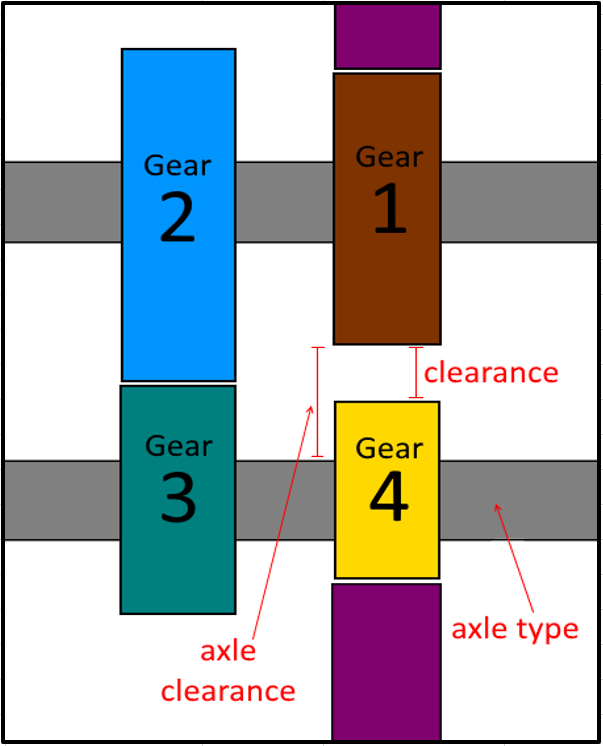
\includegraphics[width=0.4\linewidth]{Gear_Clear}
	\end{figure}
	
	Starting with the basic equations:
	\begin{equation} \label{gear_pitch_diam}
		r_p = \frac{n}{2p}
	\end{equation}
	\begin{equation} \label{gear_outside_diam}
		r_o = \frac{n+2}{2p}
	\end{equation}
	\begin{equation} \label{axle_clear}
		C_a = r_{o2} + r_{o3} - r_{o1} - \frac{d_{axle}}{2}
	\end{equation}
	\begin{equation} \label{gear_clear}
		C_g = r_{o2} + r_{o3} - r_{o1} - r_{o4}
	\end{equation}
	
	\newpage
	Substituting (\ref{gear_outside_diam}) into (\ref{axle_clear}) and (\ref{gear_clear}), respectively, gives:
	\begin{equation}
		C_a = \frac{n_2 + n_3}{2 p_{23}} - \frac{n_1}{2 p_1} - \frac{d_{axle}}{2}
	\end{equation}
	\begin{equation}
		C_g = \frac{n_2 + n_3}{2 p_{23}} - \frac{n_1}{2 p_1} - \frac{n_4}{2 p_4}
	\end{equation}
	The axle or gear clears if $C_a > 0$ or $C_g > 0$, respectively. \\ \\
	$C_a$ = Axle Clearance \\
	$C_g$ = Gear Clearance \\
	$r_p$ = Pitch Radius \\
	$r_o$ = Outside Radius \\
	$n$ = \# of Teeth \\
	$p$ = Diametrical Pitch (a.k.a. dp)\\
	$d_{axle}$ = Axle Diameter
	
	\bigskip
	\section{Ratio \& Distance Calculator}
	We have the basic equations:
	\begin{equation}
		G = \frac{N}{n}
	\end{equation}
	\begin{equation}
		d = \frac{N + n}{2 p}
	\end{equation}
	
	Solving these equations for $n$ and $N$ gives:
	\begin{equation}
		n = \frac{2 d p}{G + 1}
	\end{equation}
	\begin{equation}
		N = \frac{2 d p}{G + 1} G
	\end{equation}
	
	For each gear we can get the pitch diameter and outside diameter using (\ref{gear_pitch_diam}) and (\ref{gear_outside_diam}), respectively. \\ \\
	$N$ = \# of Teeth on Large Gear \\
	$n$ = \# of Teeth on Small Gear \\
	$G$ = Gear Ratio \\
	$d$ = Center-to-Center Distance \\
	$p$ = Diametrical Pitch (a.k.a. dp)\\
	
	\newpage
	\section{Pneumatics Calculator}
	The "simulation" is run at timesteps of $dt$ = 1 second for a duration of 150 seconds. \\ \\
	
	The pressure at the current step of the simulation can be calculated by:
	\begin{equation} \label{pneu_press_timestep}
		P_{n+1} = P_n + \frac{W_{comp} - \sum W_{cyl}}{V}
	\end{equation}
	\begin{equation} \label{pneu_w_comp}
		W_{comp} = \dot{V}_{comp}(P) \cdot dt \cdot 1 \text{atm}
	\end{equation}
	\begin{equation} \label{pneu_w_cyl}
		W_{cyl} = \left( \frac{\pi D^2}{4} P_{push} + \frac{\pi (D^2 - d^2)}{4} P_{pull} \right) L \cdot m
	\end{equation}
	$\dot{V}_{comp}(P)$ is the compressor flow-rate as a function of the output pressure, taken from a fourth-degree polynomial interpolation of the data provided online. The volume of air is measured at atmospheric pressure, not at system pressure. $m$ is the number of actuations per second (can be 0 when not firing, 1 when firing, or $m>1$ if firing more than once per second). \\
	
	Derivations of these equations can be found in Appendix \ref{appendixE}. \\
	
	We can also calculate the pushing and pulling force of each cylinder using the formulas:
	\begin{equation}
		F_{push} = \frac{\pi D^2}{4} P_{push}
	\end{equation}
	\begin{equation}
		F_{pull} = \frac{\pi (D^2 - d^2)}{4} P_{pull}
	\end{equation}
	$P_n$ = System Pressure at Step $n$\\
	$V$ = System Volume \\
	$W_{comp}$ = Work Done by the Compressor \\
	$W_{cyl}$ = Work Done by Each Cylinder \\
	$D$ = Cylinder Diameter \\
	$d$ = Cylinder Rod Diameter \\
	$L$ = Cylinder Length \\
	$P_{push}$ = Pushing Pressure \\
	$P_{pull}$ = Pulling Pressure \\
	$F_{push}$ = Pushing Force \\
	$F_{pull}$ = Pulling Force
	
	\newpage
	\section{Pneumatic Linkage Calculator}
	\begin{figure}[H]
		\centering
		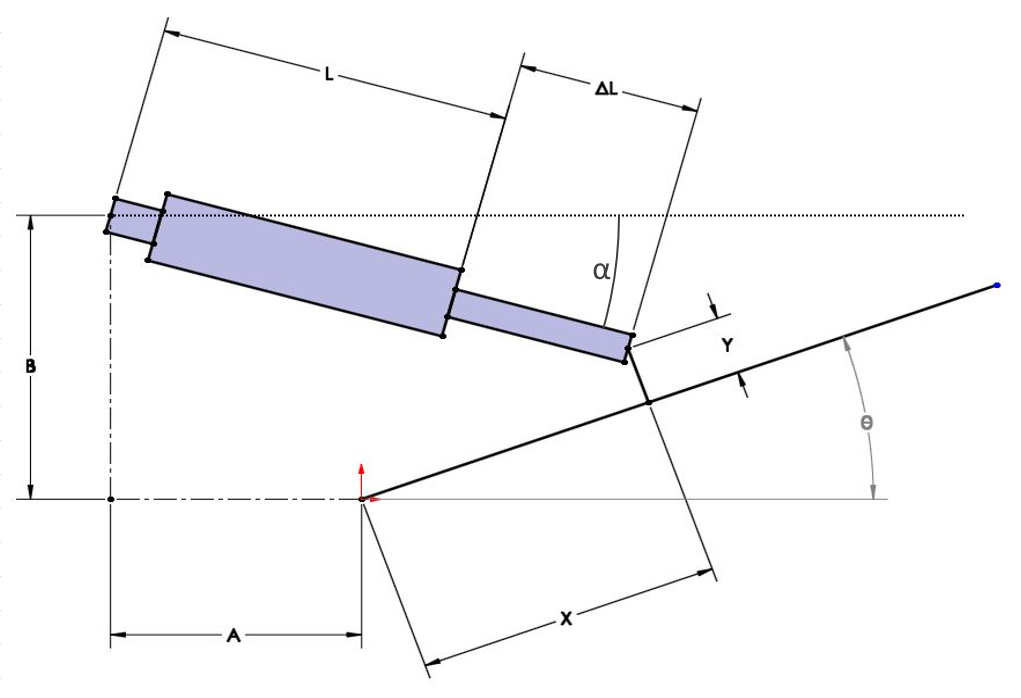
\includegraphics[width=0.8\linewidth]{Pneu_Link}
	\end{figure}
	
	Let $\theta_1$ and $\alpha_1$ represent the system when the cylinder is retracted, and $\theta_2$ and $\alpha_2$ represent it when extended. \\ \\
	
	In the horizontal direction we have:
	\begin{equation} \label{link_x_ret}
		A + X \cos \theta_1 - Y \sin \theta_1 = L \cos \alpha_1
	\end{equation}
	\begin{equation} \label{link_x_ext}
		A + X \cos \theta_2 - Y \sin \theta_2 = (L + \Delta L) \cos \alpha_2
	\end{equation}
	
	And in the vertical direction we have:
	\begin{equation} \label{link_y_ret}
		X \sin \theta_1 + Y \cos \theta_1 = B - L \sin \alpha_1
	\end{equation}
	\begin{equation} \label{link_y_ext}
		X \sin \theta_2 + Y \cos \theta_2 = B - (L + \Delta L) \sin \alpha_2
	\end{equation}
	
	We can combine (\ref{link_x_ret}) and (\ref{link_y_ext}) to remove $\alpha_1$ and get:
	\begin{equation} \label{link_ret}
		L^2 = A^2 + B^2 + X^2 + Y^2 + 2AX \cos \theta_1 - 2BY \cos \theta_1 - 2BX \sin \theta_1 - 2AY \sin \theta_1
	\end{equation}
	
	And combine (\ref{link_x_ext}) and (\ref{link_y_ext}) to remove $\alpha_2$ and get:
	\begin{equation} \label{link_ext}
		(L + \Delta L)^2 = A^2 + B^2 + X^2 + Y^2 + 2AX \cos \theta_2 - 2BY \cos \theta_2 - 2BX \sin \theta_2 - 2AY \sin \theta_2
	\end{equation}
	
	To derive the forward formulas, you can solve (\ref{link_ret}) and (\ref{link_ext}) separately to get expressions for $\theta_1$ and $\theta_2$. To derive the reverse formulas, you can solve (\ref{link_ret}) and (\ref{link_ext}) as a system of equations to get expressions for $A$ and $B$. I will not include these expressions in this document, because they are extremely long.
	
	\newpage
	\appendix
	\part*{Derivations}
	\section{Maximum Efficiency Derivation} \label{appendixA}
	To find the maximum efficiency, we take the derivative of (\ref{motor_instant_eff}) and set it equal to 0:
	\begin{equation}
		0 = \frac{\partial \eta}{\partial \tau} = \frac{(\tilde{i_f} (\tau - \tilde{\tau_s})^2 - \tilde{i_s} \tau^2) \tilde{\omega_f}}{V (\tilde{i_s} \tau + \tilde{i_f} (\tilde{\tau_s} - \tau))^2}
	\end{equation}
	
	Solving for the value of $\tau$ at which $\eta$ is maximized:
	\begin{equation}
		\tau_{\eta_{max}} = \frac{\tilde{\tau_s} \sqrt{\tilde{i_f}}}{\sqrt{\tilde{i_f}} + \sqrt{\tilde{i_s}}}
	\end{equation}
	
	We know that $\tau_{manip} = G \cdot \tau_{motor}$, so we can substitute $\tau_{\eta_{max}}$ for $\tau_{motor}$:
	\begin{equation}
		G = \frac{\tau_{manip}}{\tau_{motor}} = \frac{r \cdot F}{\tau_{\eta_{max}}} = \frac{r \cdot F}{\frac{\tilde{\tau_s} \sqrt{\tilde{i_f}}}{\sqrt{\tilde{i_f}} + \sqrt{\tilde{i_s}}}}
	\end{equation}
	
	And simplifying gives:
	\begin{equation} \tag{\ref*{max_eff}}
		G = \frac{r F}{\tilde{\tau_s}} \left( 1 + \sqrt{\frac{\tilde{i_s}}{\tilde{i_f}}} \right)
	\end{equation}
	
	\bigskip
	\section{Equivalent Radius/Load Derivation} \label{appendixB}
	To find the equivalent radius, we equate the rotational $\to$ linear motion transformation equations for both a wheel (\ref{wheel_lin_rot}) and lead screw (\ref{lead_screw_lin_rot})
	\begin{equation}
		2 \pi r \cdot \omega = v = \omega \cdot n p
	\end{equation}
	
	We can then solve for $r = r_{eq}$ to find the radius that will provide the same rotational $\to$ linear motion transformation as the given lead screw
	\begin{equation} \tag{\ref*{r_eq}}
		r_{eq} = \frac{n p}{2 \pi}
	\end{equation}
	
	We want to conserve the work done by a lead screw and equivalent wheel across one rotation (where $x$ can be $L$ or $R$). 
	\begin{equation}
		W = 2 \pi r_{eq} \cdot L_{x,eq} = 2 \pi T_x
	\end{equation}
	
	Solving for $L_{x,eq}$, we get:
	\begin{equation}
		L_{x,eq} = \frac{T_x}{r_{eq}}
	\end{equation}
	
	\newpage
	\section{Projectile Equation Derivations} \label{appendixC}
	Starting with basic projectile motion equations:
	\begin{equation} \label{projX}
		\Delta x = v_i \cos \theta_i \cdot t
	\end{equation}
	\begin{equation} \label{projY}
		\Delta y = v_i \sin \theta_i \cdot t - \tfrac{1}{2} g t^2
	\end{equation}
	\begin{equation} \label{theta_f}
		\theta_f = \tan^{-1} \left( \frac{v_{f,y}}{v_{f,x}} \right) = \tan^{-1} \left( \frac{v_i \sin \theta_i - g t}{v_i \cos \theta_i} \right)
	\end{equation}
	
	Solving (\ref{projX}) for $t$ and substituting into (\ref{projY}) gives:
	\begin{equation}
		\Delta y = \Delta x \tan \theta_i - \frac{g \cdot (\Delta x)^2}{2 v_i^2 \cos^2 \theta_i}
	\end{equation}
	
	We can then substitute in $\Delta x = d$ and $\Delta y = h_f - h_i$:
	\begin{equation} \tag{\ref*{proj_final_height}}
		h_f = h_i + d \tan \theta_i - \frac{g \cdot d^2}{2 v_i^2 \cos^2 \theta_i}
	\end{equation}
	
	Solving (\ref{projX}) for $t$ and substituting into (\ref{theta_f}) gives:
	\begin{equation} \label{theta_f_solved}
		\theta_f = \tan^{-1} \left( \frac{v_i \sin \theta_i - g \cdot \frac{\Delta x}{v_i \cos \theta_i}}{v_i \cos \theta_i} \right) = \tan^{-1} \left( \tan \theta_i - \frac{g \cdot d}{v_i^2 \cos^2 \theta_i} \right)
	\end{equation}
	
	Further substituting in (\ref{proj_final_height}) into (\ref{theta_f_solved}) gives:
	\begin{equation} \label{theta_f_transform}
		\theta_f = \tan^{-1} \left( \tan \theta_i - \frac{2}{d} (d \tan \theta_i - (h_f - h_i)) \right)
	\end{equation}
	
	And by simplifying we get:
	\begin{equation} \tag{\ref*{proj_final_angle}}
		\theta_f = \tan^{-1} \left( 2 \frac{h_f - h_i}{d} - \tan \theta_i \right)
	\end{equation}
	
	To calculate the reverse equations, we can solve (\ref{theta_f_transform}) for $\theta_i$:
	\begin{equation} \tag{\ref*{proj_init_angle}}
		\theta_i = \tan^{-1} \left( 2 \frac{h_f - h_i}{d} - \tan \theta_f \right)
	\end{equation}
	
	Then substitute (\ref{proj_final_height}) into (\ref{proj_init_angle}):
	\begin{equation}
		\tan \theta_i + \tan \theta_f = \frac{2}{d} \left( d \tan \theta_i - \frac{g \cdot d^2}{2 v_i^2 \cos^2 \theta_i} \right)
	\end{equation}
	
	And solve that for $v_i$:
	\begin{equation} \tag{\ref*{proj_init_vel}}
		v_i = \sec \theta_i \cdot \sqrt{\frac{g \cdot d}{\left| \tan \theta_i - \tan \theta_f \right|}}
	\end{equation}
	
	\section{Chain Length Derivation} \label{appendixD}

	\begin{figure}[H]
		\centering
		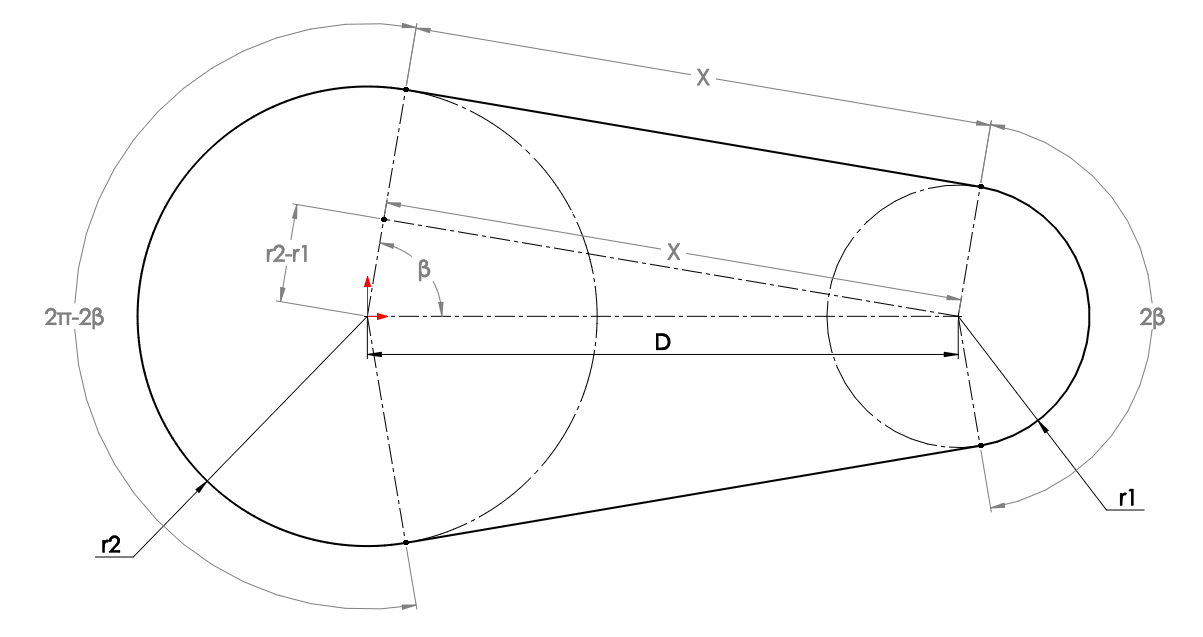
\includegraphics[width=\linewidth]{Chain_Derivation}
	\end{figure}
	
	It is clear that:
	\begin{equation} \label{chain_L_general}
		L = 2 X + r_1 \cdot 2 \beta + r_2 \cdot (2 \pi - 2 \beta)
	\end{equation}
	
	Looking at the right triangle in the center of the image, we can see that:
	\begin{equation} \label{chain_X}
		D^2 = X^2 + (r_2 - r_1)^2 \implies X = \sqrt{D^2 - (r_1 - r_2)^2}
	\end{equation}
	\begin{equation} \label{chain_beta}
		\beta = \cos^{-1} \left( \frac{r_2 - r_1}{D} \right) = \cos^{-1} \left( \frac{r_1 - r_2}{D} \right)
	\end{equation}
	
	Substituting (\ref{chain_X}) and (\ref{chain_beta}) into (\ref{chain_L_general}) gives:
	\begin{equation}
		L = 2 \sqrt{D^2 - (r_1 - r_2)^2} + r_1 \cdot 2 \cos^{-1} \left( \frac{r_1 - r_2}{D} \right) + r_2 \cdot \left( 2 \pi - 2 \cos^{-1} \left( \frac{r_1 - r_2}{D} \right) \right)
	\end{equation}
	
	And rearranging gives:
	\begin{equation} \tag{\ref*{chain_len}}
		L = 2 \sqrt{D^2 - (r_1 - r_2)^2} + 2 (r_1 - r_2) \cos^{-1} \left( \frac{r_1 - r_2}{D} \right) + 2 \pi r_2
	\end{equation}
	
	\newpage
	\section{Pneumatics Simulation Derivation} \label{appendixE}
	We know that the energy of the system at any point can be represented by:
	\begin{equation} \label{pneu_energy_basic}
		E = P \cdot V
	\end{equation}
	
	We can find the energy of the system at any timestep by adding the total work done on the system in that time to the energy of the system at the previous step:
	\begin{equation} \label{pneu_energy_timestep}
		E_{n+1} = E_n + W_{tot}
	\end{equation}
	
	Substituting (\ref{pneu_energy_basic}) into (\ref{pneu_energy_timestep}) gives:
	\begin{equation}
		(PV)_{n+1} = (PV)_n + W_{comp} - \sum W_{cyl}
	\end{equation}
	
	Since the volume of the system remains constant, we can divide by $V$ to get:
	\begin{equation} \tag{\ref*{pneu_press_timestep}}
		P_{n+1} = P_n + \frac{W_{comp} - \sum W_{cyl}}{V}
	\end{equation}
	
	Basic thermodynamics says that the work done by compression/expansion of gas at constant pressure can be represented by $W = P \cdot \Delta V$. In each actuation of a cylinder gas is compressed twice, once for extension and once for retraction. So for each timestep, the work done on the cylinder can be expressed as:
	\begin{equation}
		W_{cyl} = ((PAL)_{push} + (PAL)_{pull}) \cdot m
	\end{equation}
	
	$L$ is constant, so it can be factored out. We can also substitute $A$ for the effective piston areas, giving:
	\begin{equation} \tag{\ref*{pneu_w_cyl}}
		W_{cyl} = \left( \frac{\pi D^2}{4} P_{push} + \frac{\pi (D^2 - d^2)}{4} P_{pull} \right) L \cdot m
	\end{equation}
	
	Similarly, we can represent the work done by the compressor as:
	\begin{equation} \tag{\ref*{pneu_w_comp}}
		W_{comp} = \dot{V}_{comp}(P) \cdot dt \cdot 1 \text{atm}
	\end{equation}
	Note: since $\dot{V}_{comp}$ is measured at atmospheric pressure, $P$ must be 1 atm and not the system pressure
	
\end{document}